%!TeX encoding = UTF-8
\documentclass[notheorems, aspectratio=54]{beamer}
% aspectratio: 1610, 149, 54, 43(default), 32
\usepackage[utf8]{inputenc}
\usepackage[english, vietnamese]{babel}
\usepackage{latexsym}
\usepackage{amsmath,amssymb}
\usepackage{mathtools}
\usepackage{color,xcolor}
\usepackage{graphicx}
\usepackage{algorithm}
\usepackage{amsthm}
\usepackage{lmodern} % 解决 font warning
% \usepackage[UTF8]{ctex}
\usepackage{animate} % insert gif

\usepackage{lipsum} % To generate test text 
\usepackage{ulem} % 下划线,波浪线

\usepackage{listings} % display code on slides; don't forget [fragile] option after \begin{frame}

% ----------------------------------------------
% tikx
\usepackage{framed}
\usepackage{tikz}
\usepackage{pgf}
\usetikzlibrary{calc,trees,positioning,arrows,chains,shapes.geometric,%
	decorations.pathreplacing,decorations.pathmorphing,shapes,%
	matrix,shapes.symbols}
\pgfmathsetseed{1} % To have predictable results
% Define a background layer, in which the parchment shape is drawn
\pgfdeclarelayer{background}
\pgfsetlayers{background,main}

% define styles for the normal border and the torn border
\tikzset{
	normal border/.style={orange!30!black!10, decorate, 
		decoration={random steps, segment length=2.5cm, amplitude=.7mm}},
	torn border/.style={orange!30!black!5, decorate, 
		decoration={random steps, segment length=.5cm, amplitude=1.7mm}}}

% Macro to draw the shape behind the text, when it fits completly in the
% page
\def\parchmentframe#1{
	\tikz{
		\node[inner sep=2em] (A) {#1};  % Draw the text of the node
		\begin{pgfonlayer}{background}  % Draw the shape behind
			\fill[normal border] 
			(A.south east) -- (A.south west) -- 
			(A.north west) -- (A.north east) -- cycle;
\end{pgfonlayer}}}

% Macro to draw the shape, when the text will continue in next page
\def\parchmentframetop#1{
	\tikz{
		\node[inner sep=2em] (A) {#1};    % Draw the text of the node
		\begin{pgfonlayer}{background}    
			\fill[normal border]              % Draw the ``complete shape'' behind
			(A.south east) -- (A.south west) -- 
			(A.north west) -- (A.north east) -- cycle;
			\fill[torn border]                % Add the torn lower border
			($(A.south east)-(0,.2)$) -- ($(A.south west)-(0,.2)$) -- 
			($(A.south west)+(0,.2)$) -- ($(A.south east)+(0,.2)$) -- cycle;
\end{pgfonlayer}}}

% Macro to draw the shape, when the text continues from previous page
\def\parchmentframebottom#1{
	\tikz{
		\node[inner sep=2em] (A) {#1};   % Draw the text of the node
		\begin{pgfonlayer}{background}   
			\fill[normal border]             % Draw the ``complete shape'' behind
			(A.south east) -- (A.south west) -- 
			(A.north west) -- (A.north east) -- cycle;
			\fill[torn border]               % Add the torn upper border
			($(A.north east)-(0,.2)$) -- ($(A.north west)-(0,.2)$) -- 
			($(A.north west)+(0,.2)$) -- ($(A.north east)+(0,.2)$) -- cycle;
\end{pgfonlayer}}}

% Macro to draw the shape, when both the text continues from previous page
% and it will continue in next page
\def\parchmentframemiddle#1{
	\tikz{
		\node[inner sep=2em] (A) {#1};   % Draw the text of the node
		\begin{pgfonlayer}{background}   
			\fill[normal border]             % Draw the ``complete shape'' behind
			(A.south east) -- (A.south west) -- 
			(A.north west) -- (A.north east) -- cycle;
			\fill[torn border]               % Add the torn lower border
			($(A.south east)-(0,.2)$) -- ($(A.south west)-(0,.2)$) -- 
			($(A.south west)+(0,.2)$) -- ($(A.south east)+(0,.2)$) -- cycle;
			\fill[torn border]               % Add the torn upper border
			($(A.north east)-(0,.2)$) -- ($(A.north west)-(0,.2)$) -- 
			($(A.north west)+(0,.2)$) -- ($(A.north east)+(0,.2)$) -- cycle;
\end{pgfonlayer}}}

% Define the environment which puts the frame
% In this case, the environment also accepts an argument with an optional
% title (which defaults to ``Example'', which is typeset in a box overlaid
% on the top border
\newenvironment{parchment}[1][Example]{%
	\def\FrameCommand{\parchmentframe}%
	\def\FirstFrameCommand{\parchmentframetop}%
	\def\LastFrameCommand{\parchmentframebottom}%
	\def\MidFrameCommand{\parchmentframemiddle}%
	\vskip\baselineskip
	\MakeFramed {\FrameRestore}
	\noindent\tikz\node[inner sep=1ex, draw=black!20,fill=white, 
	anchor=west, overlay] at (0em, 2em) {\sffamily#1};\par}%
{\endMakeFramed}

% ----------------------------------------------

\mode<presentation>{
	\usetheme{CambridgeUS}
	% Boadilla CambridgeUS
	% default Antibes Berlin Copenhagen
	% Madrid Montpelier Ilmenau Malmoe
	% Berkeley Singapore Warsaw
	\usecolortheme{beaver}
	% beetle, beaver, orchid, whale, dolphin
	\useoutertheme{infolines}
	% infolines miniframes shadow sidebar smoothbars smoothtree split tree
	\useinnertheme{circles}
	% circles, rectanges, rounded, inmargin
}
% 设置 block 颜色
\setbeamercolor{block title}{bg=red!30,fg=white}

\newcommand{\reditem}[1]{\setbeamercolor{item}{fg=red}\item #1}

% 缩放公式大小
\newcommand*{\Scale}[2][4]{\scalebox{#1}{\ensuremath{#2}}}

% 解决 font warning
\renewcommand\textbullet{\ensuremath{\bullet}}

% ---------------------------------------------------------------------
% flow chart
\tikzset{
	>=stealth',
	punktchain/.style={
		rectangle, 
		rounded corners, 
		% fill=black!10,
		draw=white, very thick,
		text width=6em,
		minimum height=2em, 
		text centered, 
		on chain
	},
	largepunktchain/.style={
		rectangle,
		rounded corners,
		draw=white, very thick,
		text width=10em,
		minimum height=2em,
		on chain
	},
	line/.style={draw, thick, <-},
	element/.style={
		tape,
		top color=white,
		bottom color=blue!50!black!60!,
		minimum width=6em,
		draw=blue!40!black!90, very thick,
		text width=6em, 
		minimum height=2em, 
		text centered, 
		on chain
	},
	every join/.style={->, thick,shorten >=1pt},
	decoration={brace},
	tuborg/.style={decorate},
	tubnode/.style={midway, right=2pt},
	font={\fontsize{10pt}{12}\selectfont},
}
% ---------------------------------------------------------------------

% code setting
\lstset{
	language=C++,
	basicstyle=\ttfamily\footnotesize,
	keywordstyle=\color{red},
	breaklines=true,
	xleftmargin=2em,
	numbers=left,
	numberstyle=\color[RGB]{222,155,81},
	frame=leftline,
	tabsize=4,
	breakatwhitespace=false,
	showspaces=false,               
	showstringspaces=false,
	showtabs=false,
	morekeywords={Str, Num, List},
}


%
\author{Vương Gia Bảo, Nguyễn Viết Dũng\newline Ngô Xuân Kiên, Lê Nhựt Nam}
\title{NHẬP MÔN MÁY HỌC \newline SPEAKER RECOGNITION FROM \newline RAW WAVEFORM WITH SINCNET}


%
\setbeamertemplate{caption}[numbered]
% \setbeamertemplate{footline}[frame number]
% footer
\makeatletter
\setbeamertemplate{footline}
{
	\leavevmode%
	\hbox{%
		\begin{beamercolorbox}[wd=1\paperwidth,ht=2.25ex,dp=1ex,right]{institute in head/foot}%
			\usebeamerfont{title in head/foot} 
			\insertframenumber{} / \inserttotalframenumber\hspace*{2ex} 
	\end{beamercolorbox}}%
}
\makeatother
%
\newcommand{\argmax}{\arg\!\max}

\begin{document}

\begin{frame}
	\centering
	ĐẠI HỌC QUỐC GIA THÀNH PHỐ HỒ CHÍ MINH
	
	ĐẠI HỌC KHOA HỌC TỰ NHIÊN
	
	KHOA CÔNG NGHỆ THÔNG TIN - BỘ MÔN KHOA HỌC MÁY TÍNH
	\titlepage
\end{frame}

\begin{frame}{Nội dung trình bày}
\tableofcontents
\end{frame}
\section{Chuẩn bị dữ liệu - Data Preparation}
\subsection{Về \textbf{Tiếng Anh}}
\begin{frame}{Chuẩn bị dữ liệu}
	Về \textbf{Tiếng Anh}
	\begin{itemize}
		\item Với TIMIT, ta có một kho ngữ liệu với 462 người nói, các khoảng không phải lời nói ở đầu và cuối mỗi câu đã bị xóa, những tập tin về nội dung câu nói của TIMIT cũng được loại bỏ. Sau khi tinh chỉnh toàn bộ dữ liệu, nhóm dùng 5 câu nói của mỗi người nói để huấn luyện, 3 câu nói của mỗi người nói dùng để kiểm tra.
		\item Với LibriSpeech, những phần với độ im lặng bên trong kéo dài hơn 125 ms được
		chia thành nhiều phần nhỏ. Việc chia tập huấn luyện (training set), tập kiểm tra (testing set) là ngẫu nhiên bằng cách chọn 12-15 giây dữ liệu huấn luyện của mỗi người nói và các câu kiểm tra kéo dài từ 2-6 giây.
	\end{itemize}
\end{frame}
\subsection{Về \textbf{Tiếng Việt}}
\begin{frame}{Chuẩn bị dữ liệu}
	Về \textbf{Tiếng Việt}: Nhóm dùng tập dữ liệu Son et al. Dataset
	\begin{itemize}
		\item Nguồn dữ liệu từ bài báo Vietnamese Speaker Authentication Using Deep Models
		\item Dung lượng của tập dữ liệu: 535 MB
		\item Số mẫu trong tập dữ liệu: 400 mẫu
		\item Bộ dữ liệu gồm: hai tập Men và Women, mỗi tập con chứa 10 thư mục người nói. Mỗi thư mục người nói chứa 20 đoạn ghi âm, chia ra Long và Short (mỗi loại 10 đoạn)
		\item Điểm hạn chế: Bộ dữ liệu có kích thước khá nhỏ
	\end{itemize}
\end{frame}
\section{Xây dựng thực nghiệm mô hình \textbf{SincNet}}
\begin{frame}{SincNet Architecture Digram}
	\begin{figure}[H]
		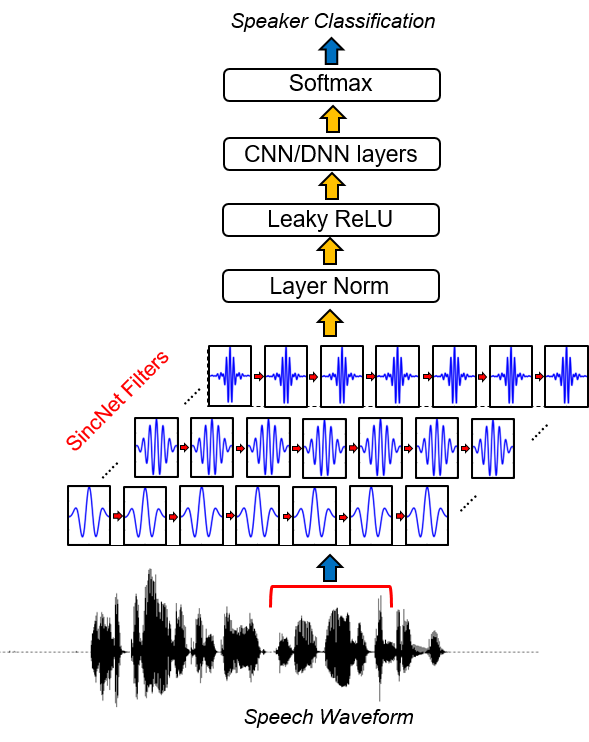
\includegraphics[width=0.4\linewidth]{images/SincNet.png}
		\caption{The SincNet Architecture}
		\label{fig:writing-thesis}
	\end{figure}
\end{frame}
\begin{frame}{Speaker Recognition Pipeline}
	\begin{figure}[H]
		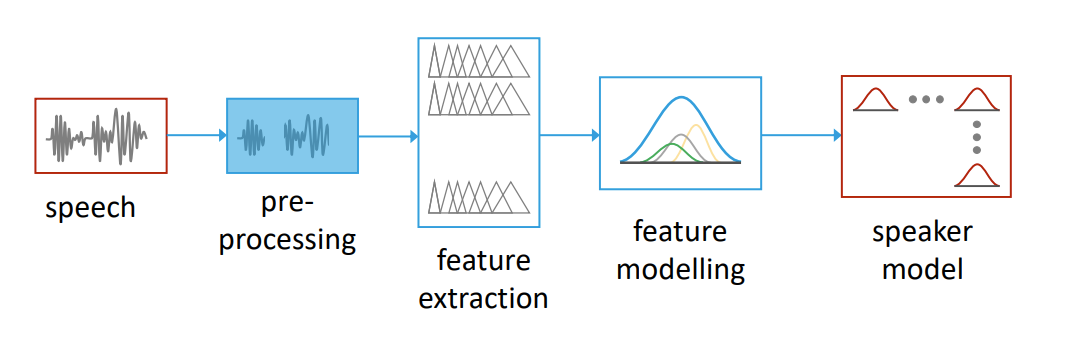
\includegraphics[width=0.95\linewidth]{images/speaker_recognition_pipeline.png}
		\caption{Speaker Recognition Pipeline}
		\label{fig:writing-thesis}
	\end{figure}
\end{frame}
\subsection{Xây dựng thực nghiệm với \textbf{tiếng Anh}}
\begin{frame}{Sử dụng tập dữ liệu TIMIT}
	Các thông số mô hình khi sử dụng tập TIMIT
	\begin{itemize}
		\item Các cửa sổ có $\text{fs} = 16000$, tín hiệu được cắt thành những chunks với $\text{cw\_len}=200$, overlap $\text{cw\_shift}=10$s
		\item Lớp Input: sử dụng 80 bộ lọc SincNet có kích thước $L=251$, max pool - 3, sử dụng Layer Norm cho cả input và output, không dùng Batch Norm, hàm kích hoạt activation leaky-ReLU, dropout = 0
		\item Hai lớp CNN: sử dụng 2 lớp CNN, với mỗi lớp dùng 60 bộ lọc có kích thuốc $L=5$, sử dụng Layer Norm cho cả input và output, không dùng Batch Norm, hàm kích hoạt activation leaky-ReLU, dropout = 0
		\item Ba lớp DNN: sử dụng 3 lớp DNN (Multi Layer Perceptron) fully-connected với 2048 neurons, Layer Norm cho input, Batch Norm cho output, các lớp ẩn (hidden layers) dùng leaky-ReLU
		\item Lớp Output: Multi Layer Perceptron, 462 nodes, không dropout, không LayerNorm, không BatchNorm cho cả input và output, hàm activation function dùng softmax 
	\end{itemize}
\end{frame}
\begin{frame}{Sử dụng tập dữ liệu TIMIT}
	Các Hyper parameters
	\begin{itemize}
		\item learning rate $\text{lr} = 0.001$
		\item $\alpha = 0.95$
		\item $\epsilon = 10^{-7}$
		\item $\text{batch\_size}=128$
		\item $\text{N\_epochs}=100$
		\item $\text{N\_batches}=800$
		\item $\text{N\_eval\_epoch}=8$
		\item $\text{seed}=1234$
	\end{itemize}
\end{frame}
\begin{frame}{Sử dụng tập dữ liệu Librispeech}
	Các thông số mô hình khi sử dụng tập Librispeech
	\begin{itemize}
		\item Các cửa sổ có $\text{fs} = 8000$, tín hiệu được cắt thành những chunks với $\text{cw\_len}=375$, overlap $\text{cw\_shift}=10$s
		\item Lớp Input: sử dụng 80 bộ lọc SincNet có kích thước $L=251$, max pool - 3, sử dụng Layer Norm cho cả input và output, không dùng Batch Norm, hàm kích hoạt activation leaky-ReLU, dropout = 0
		\item Hai lớp CNN: sử dụng 2 lớp CNN, với mỗi lớp dùng 60 bộ lọc có kích thuốc $L=5$, sử dụng Layer Norm cho cả input và output, không dùng Batch Norm, hàm kích hoạt activation leaky-ReLU, dropout = 0
		\item Hai lớp DNN: sử dụng 2 lớp DNN (Multi Layer Perceptron) fully-connected với 2048 neurons, Layer Norm cho input, Batch Norm cho output, các lớp ẩn (hidden layers) dùng leaky-ReLU làm activation cho lớp DNN thứ nhất, lớp kia dùng linear
		\item Lớp Output: 2 lớp Multi Layer Perceptron, 2048 nodes cho mỗi lớp, không dropout, Layer Norm cho input, Batch Norm cho output, hàm activation function lớp thứ nhất dùng leaky-ReLU, lớp thứ hai dùng softmax
	\end{itemize}
\end{frame}
\begin{frame}{Sử dụng tập dữ liệu Librispeech}
		Các Hyper parameters
		\begin{itemize}
			\item \item learning rate $\text{lr} = 0.001$
			\item $\alpha = 0.95$
			\item $\epsilon = 10^{-7}$
			\item $\text{batch\_size}=128$
			\item $\text{N\_epochs}=100$
			\item $\text{N\_batches}=100$
			\item $\text{N\_eval\_epoch}=10$
			\item $\text{reg\_factor}=1000$
			\item $\text{fact\_amp=0.2}$
			\item $\text{seed}=1234$
		\end{itemize}
\end{frame}
\subsection{Xây dựng thực nghiệm với \textbf{tiếng Việt}}
\begin{frame}{Sử dụng tập dữ liệu Son et al. Dataset}
	Các thông số mô hình khi sử dụng tập Son et al. Dataset
	\begin{itemize}
		\item Các cửa sổ có $\text{fs} = 16000$, tín hiệu được cắt thành những chunks với $\text{cw\_len}=200$, overlap $\text{cw\_shift}=10$s
		\item Lớp Input: sử dụng 80 bộ lọc SincNet có kích thước $L=251$, max pool - 3, sử dụng Layer Norm cho cả input và output, không dùng Batch Norm, hàm kích hoạt activation leaky-ReLU, dropout = 0
		\item Hai lớp CNN: sử dụng 2 lớp CNN, với mỗi lớp dùng 60 bộ lọc có kích thuốc $L=5$, sử dụng Layer Norm cho cả input và output, không dùng Batch Norm, hàm kích hoạt activation leaky-ReLU, dropout = 0
		\item Ba lớp DNN: sử dụng 3 lớp DNN (Multi Layer Perceptron) fully-connected với 2048 neurons, Layer Norm cho input, Batch Norm cho output, các lớp ẩn (hidden layers) dùng leaky-ReLU
		\item Lớp Output: Multi Layer Perceptron, 18 nodes, không dropout, không LayerNorm, không BatchNorm cho cả input và output, hàm activation function dùng softmax
	\end{itemize}
\end{frame}
\begin{frame}{Sử dụng tập dữ liệu Son et al. Dataset}
	Các Hyper parameters
	\begin{itemize}
		\item Tốc độ học - learning rate $\text{lr} = 0.001$
		\item $\alpha = 0.95$
		\item $\epsilon = 10^{-7}$
		\item Kích thước batch norm $\text{batch\_size}=128$
		\item Số lượng epochs training $\text{N\_epochs}=300$
		\item Số lượng batch $\text{N\_batches}=100$
		\item Số đánh giá mỗi epoch $\text{N\_eval\_epoch}=1$
		\item $\text{seed}=1234$
	\end{itemize}
\end{frame}
\section{Đăng ký - Enrollment}
\subsection{Đăng ký mô hình \textbf{tiếng Anh}}
\begin{frame}{Tính toán d-vector}
	Thông số mô hình tính toán d-vector
\end{frame}
\begin{frame}{So sánh hai d-vector}
	Triển khai sử dụng độ đo cosine trong so sánh d-vector và phân ngưỡng
\end{frame}
\begin{frame}{Dự đoán từ mô hình}
	
\end{frame}
\subsection{Đăng ký mô hình \textbf{tiếng Việt}}
\begin{frame}{Tính toán d-vector}
		Thông số mô hình tính toán d-vector
\end{frame}
\begin{frame}{So sánh hai d-vector}
	Triển khai sử dụng độ đo cosine trong so sánh d-vector và phân ngưỡng
\end{frame}
\begin{frame}{Dự đoán từ mô hình}
	
\end{frame}
\section{Đánh giá mô hình}
\subsection{Đánh giá mô hình \textbf{tiếng Anh}}
\begin{frame}{Kết quả đánh giá mô hình}
	Các kết quả khi đánh giá mô hình bằng tập TIMIT
	\begin{itemize}
		\item Độ lỗi huấn luyện trung bình mỗi frame $loss\_tr=4.217127$
		\item Giá trị phân lớp sai mức frame $err\_te=0.513561$
		\item Giá trị phân lớp sai mức câu $err\_te\_snt =0.018038$
	\end{itemize}
\end{frame}
\begin{frame}{TIMIT Training Result Visualization}
	\begin{figure}[H]
		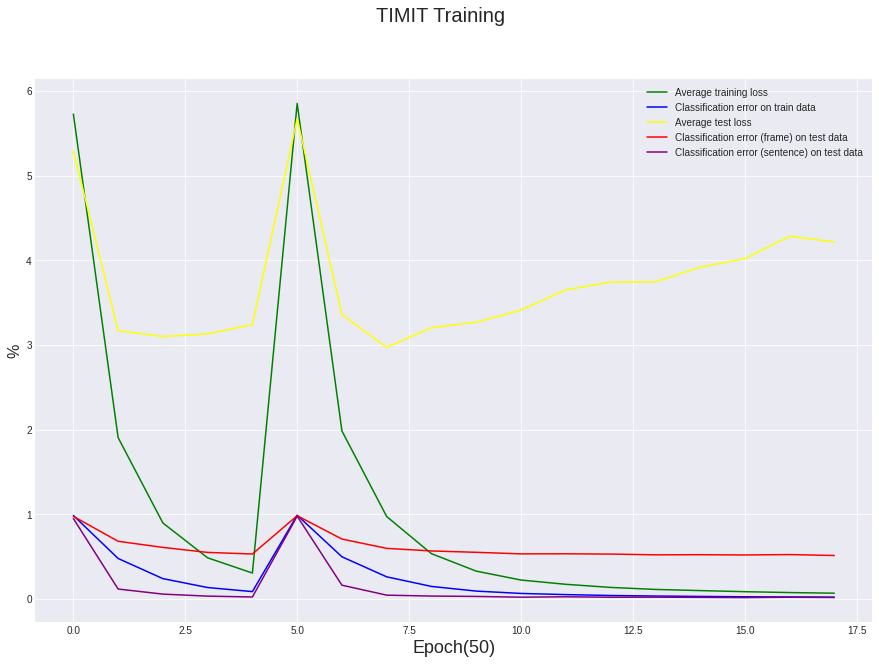
\includegraphics[width=0.8\linewidth]{result/sincnet_timit_plot.png}
		\label{fig:writing-thesis}
	\end{figure}
\end{frame}
\begin{frame}{Kết quả đánh giá mô hình}
	Các kết quả khi đánh giá mô hình bằng tập Librispeech
	\begin{itemize}
		\item Độ lỗi huấn luyện trung bình mỗi frame $loss\_tr=5.448840$
		\item Giá trị phân lớp sai mức frame $err\_te=0.907977$
		\item Giá trị phân lớp sai mức câu $err\_te\_snt =0.456924$
	\end{itemize}
\end{frame}
\begin{frame}{Librispeech Training Result Visualization}
	\begin{figure}[H]
		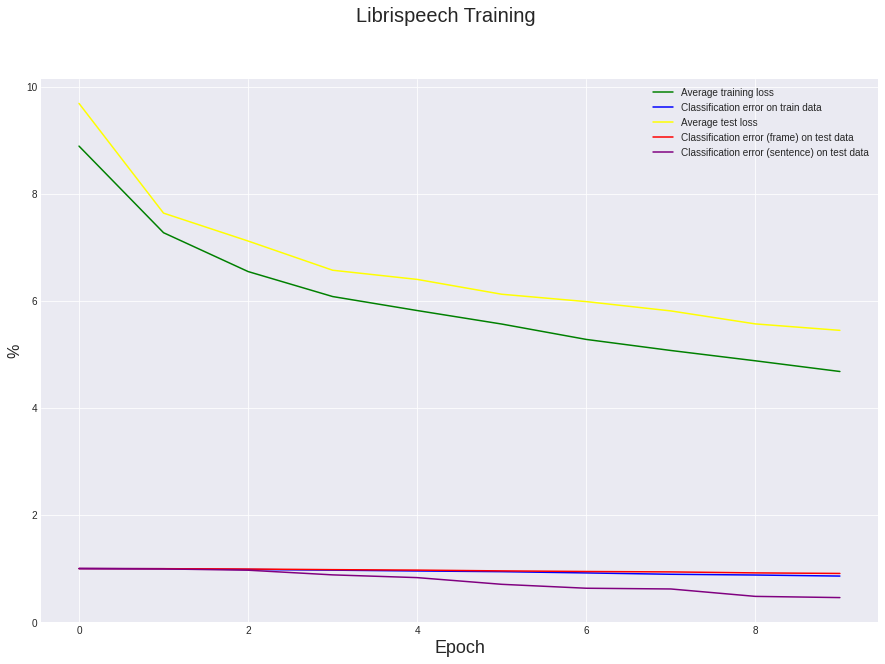
\includegraphics[width=0.8\linewidth]{result/sincnet_librispeech_plot.png}
		\label{fig:writing-thesis}
	\end{figure}
\end{frame}
\subsection{Đánh giá mô hình \textbf{tiếng Việt}}
\begin{frame}{Kết quả đánh giá mô hình}
	Các kết quả khi đánh giá mô hình bằng tập Son et al. Dataset
	\begin{itemize}
		\item Độ lỗi huấn luyện trung bình mỗi frame $loss\_tr=0.113859$
		\item Giá trị phân lớp sai mức frame $err\_te=0.031011$
		\item Giá trị phân lớp sai mức câu $err\_te\_snt =0.000000$
	\end{itemize}
\end{frame}
\begin{frame}{Son et al. Dataset Training Result Visualization}
	\begin{figure}[H]
		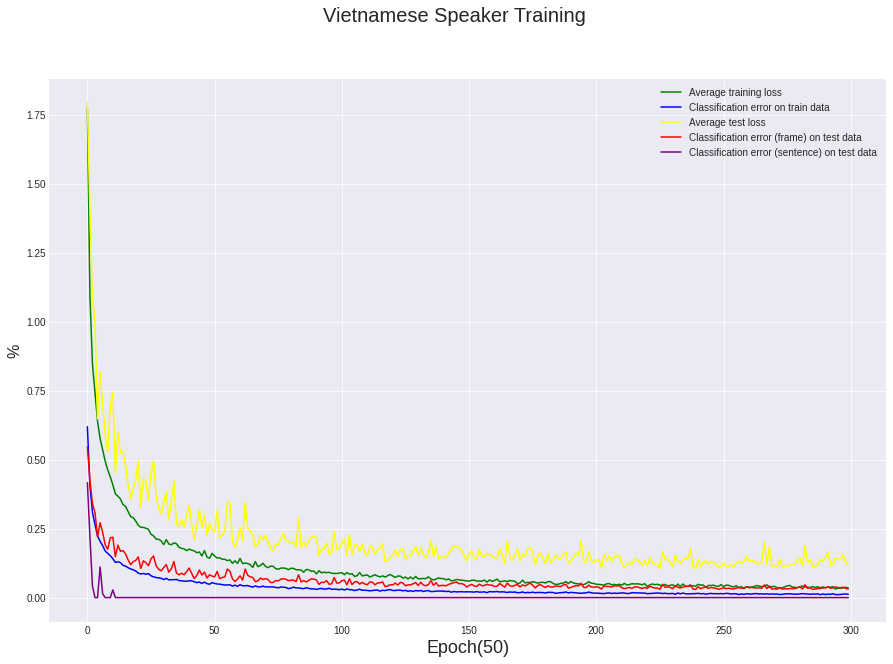
\includegraphics[width=0.8\linewidth]{result/sincnet_vietnamese_plot.png}
		\label{fig:writing-thesis}
	\end{figure}
\end{frame}
\section{Kết luận}

\section{Tài liệu tham khảo}
\begin{frame}{Tài liệu tham khảo}
	\nocite{*}
	\bibliography{references}\newpage\cleardoublepage
	\bibliographystyle{plain}
\end{frame}


\begin{frame}{Q\&A}
	\begin{center}
		\Huge Cảm ơn thầy và các bạn đã theo dõi và lắng nghe
	\end{center}
\end{frame}

\end{document}